\definecolor{initColor}{RGB}{137,135,129}
\definecolor{finalColor}{RGB}{42,120,214}
\definecolor{trainColor}{RGB}{27,175,122}
\definecolor{valColor}{RGB}{235,104,52}
\begin{figure}[htbp]
\centering
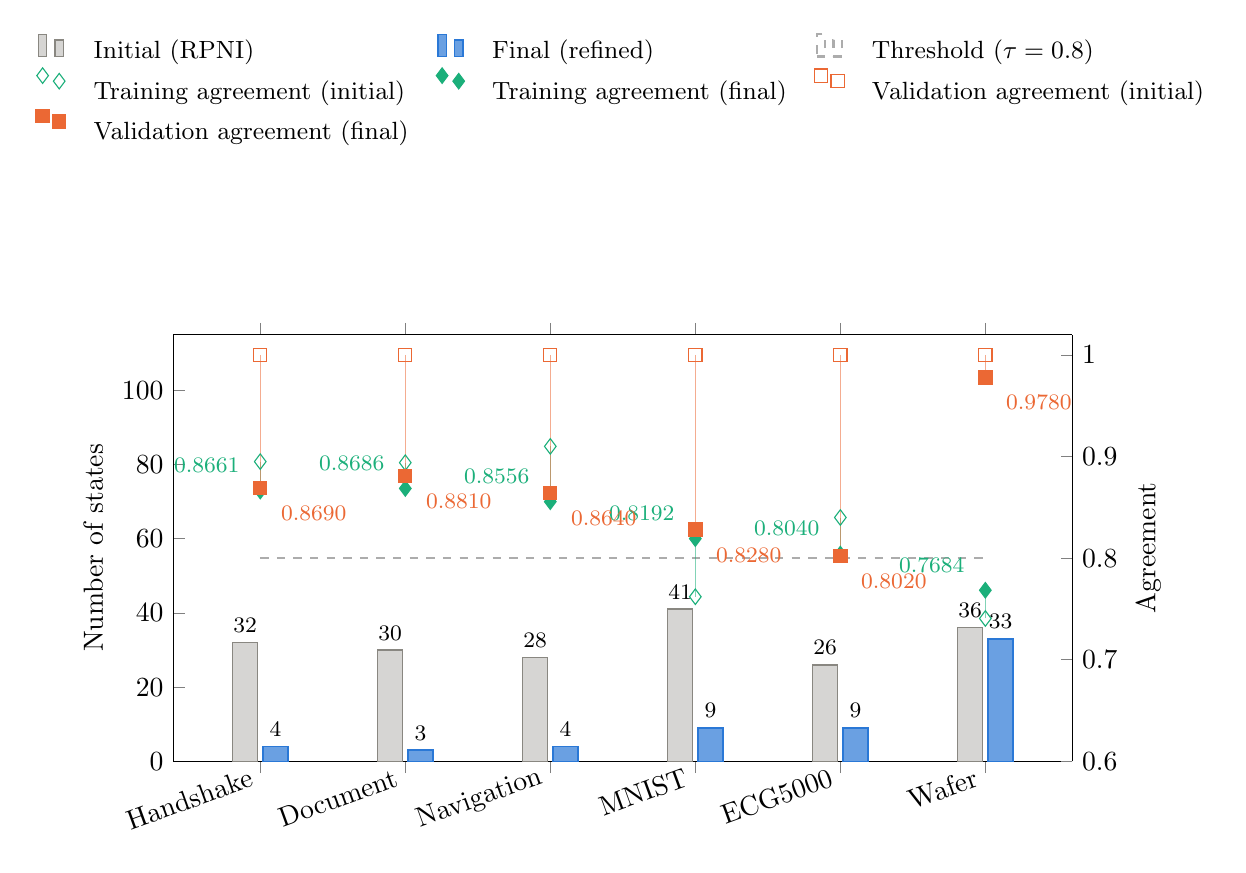
\begin{tikzpicture}
% ===== Left axis: initial and final states =====
% Carries the ONE combined legend for both axes: two overlaid axes each
% positioning their own legend via `at=` fight over the same coordinate
% space and silently clobber each other, so the right axis's series get
% phantom \addlegendimage entries here instead of a legend of their own.
\begin{axis}[
    width=13cm, height=7cm,
    ybar,
    bar width=9pt,
    axis y line*=left,
    ylabel={Number of states},
    ymin=0, ymax=115,
    symbolic x coords={Handshake,Document,Navigation,MNIST,ECG5000,Wafer},
    xtick=data,
    x tick label style={rotate=20, anchor=east},
    enlarge x limits=0.12,
    legend style={at={(0.5,1.42)}, anchor=south, legend columns=3, draw=none, font=\small, column sep=8pt},
    legend cell align=left,
    nodes near coords,
    every node near coord/.append style={font=\footnotesize},
]
\addplot[fill=initColor!35!white, draw=initColor, line width=0.5pt] coordinates {(Handshake,32) (Document,30) (Navigation,28) (MNIST,41) (ECG5000,26) (Wafer,36)};
\addlegendentry{Initial (RPNI)}
\addplot[fill=finalColor!70!white, draw=finalColor, line width=0.5pt] coordinates {(Handshake,4) (Document,3) (Navigation,4) (MNIST,9) (ECG5000,9) (Wafer,33)};
\addlegendentry{Final (refined)}
\addlegendimage{gray!65, dashed, line width=0.8pt}
\addlegendentry{Threshold ($\tau=0.8$)}
\addlegendimage{only marks, color=trainColor, mark=diamond, mark size=2.8pt}
\addlegendentry{Training agreement (initial)}
\addlegendimage{only marks, color=trainColor, mark=diamond*, mark size=2.8pt}
\addlegendentry{Training agreement (final)}
\addlegendimage{only marks, color=valColor, mark=square, mark size=2.4pt}
\addlegendentry{Validation agreement (initial)}
\addlegendimage{only marks, color=valColor, mark=square*, mark size=2.4pt}
\addlegendentry{Validation agreement (final)}
\end{axis}

% ===== Right axis: training / validation agreement, before vs. after =====
% Hollow marker = initial (origin RPNI automaton), filled marker = final
% (after refinement); the thin connecting segment makes the before/after
% change at each task read the same way the states bars do on the left axis.
\begin{axis}[
    width=13cm, height=7cm,
    axis y line*=right,
    axis x line=none,
    ylabel={Agreement},
    ymin=0.6, ymax=1.02,
    symbolic x coords={Handshake,Document,Navigation,MNIST,ECG5000,Wafer},
    xtick=data,
    enlarge x limits=0.12,
]
\addplot[color=gray!65, dashed, line width=0.8pt, forget plot]
    coordinates {(Handshake,0.8) (Wafer,0.8)};
\addplot[trainColor, thin, opacity=0.55, forget plot] coordinates {(Handshake,0.8950) (Handshake,0.8661)};
\addplot[trainColor, thin, opacity=0.55, forget plot] coordinates {(Document,0.8940) (Document,0.8686)};
\addplot[trainColor, thin, opacity=0.55, forget plot] coordinates {(Navigation,0.9100) (Navigation,0.8556)};
\addplot[trainColor, thin, opacity=0.55, forget plot] coordinates {(MNIST,0.7620) (MNIST,0.8192)};
\addplot[trainColor, thin, opacity=0.55, forget plot] coordinates {(ECG5000,0.8400) (ECG5000,0.8040)};
\addplot[trainColor, thin, opacity=0.55, forget plot] coordinates {(Wafer,0.7406) (Wafer,0.7684)};
\addplot[valColor, thin, opacity=0.55, forget plot] coordinates {(Handshake,1.0000) (Handshake,0.8690)};
\addplot[valColor, thin, opacity=0.55, forget plot] coordinates {(Document,1.0000) (Document,0.8810)};
\addplot[valColor, thin, opacity=0.55, forget plot] coordinates {(Navigation,1.0000) (Navigation,0.8640)};
\addplot[valColor, thin, opacity=0.55, forget plot] coordinates {(MNIST,1.0000) (MNIST,0.8280)};
\addplot[valColor, thin, opacity=0.55, forget plot] coordinates {(ECG5000,1.0000) (ECG5000,0.8020)};
\addplot[valColor, thin, opacity=0.55, forget plot] coordinates {(Wafer,1.0000) (Wafer,0.9780)};
\addplot[only marks, color=trainColor, mark=diamond, mark size=2.8pt, forget plot]
    coordinates {(Handshake,0.8950) (Document,0.8940) (Navigation,0.9100) (MNIST,0.7620) (ECG5000,0.8400) (Wafer,0.7406)};
\addplot[only marks, color=valColor, mark=square, mark size=2.4pt, forget plot]
    coordinates {(Handshake,1.0000) (Document,1.0000) (Navigation,1.0000) (MNIST,1.0000) (ECG5000,1.0000) (Wafer,1.0000)};
\addplot[only marks, color=trainColor, mark=diamond*, mark size=2.8pt, forget plot,
    nodes near coords={\pgfmathprintnumber[fixed, fixed zerofill, precision=4]{\pgfplotspointmeta}},
    every node near coord/.append style={font=\footnotesize, text=trainColor, anchor=south east, xshift=-4pt, yshift=3pt}]
    coordinates {(Handshake,0.8661) (Document,0.8686) (Navigation,0.8556) (MNIST,0.8192) (ECG5000,0.8040) (Wafer,0.7684)};
\addplot[only marks, color=valColor, mark=square*, mark size=2.4pt, forget plot,
    nodes near coords={\pgfmathprintnumber[fixed, fixed zerofill, precision=4]{\pgfplotspointmeta}},
    every node near coord/.append style={font=\footnotesize, text=valColor, anchor=north west, xshift=4pt, yshift=-3pt}]
    coordinates {(Handshake,0.8690) (Document,0.8810) (Navigation,0.8640) (MNIST,0.8280) (ECG5000,0.8020) (Wafer,0.9780)};
\end{axis}
\end{tikzpicture}
\caption{Same method, before vs.\ after refinement: number of DFA states (bars) and training/validation agreement (markers) for BeamSearch across the six tasks under agreement threshold $\tau=0.8$. For agreement, hollow markers are the initial (origin RPNI) automaton and filled markers are the automaton after refinement, connected by a thin segment; the dashed line indicates the specified agreement threshold.}
\label{fig:combo-tau08}
\end{figure}
